\chapter{Технологический раздел}
\section{Выбор средств разработки}
\subsection{Выбор целевой платформы}
Программный продукт  не затачивается под работу на конкретной ОС. В качестве целевых платформ разработки были выбраны ОС Windows и Linux, Данный выбор обусловлен широкой распространенностью ОС Windows и Linux, большим количеством средств разработки для данных платформ, что дает возможность выбирать
язык программирования и сопутствующие инструменты, ориентируясь на возможность простого и надежного решения рассматриваемой
задачи, а не на ограничения целевой платформы.


\subsection{Выбор языка программирования}
Для написания комплекса программ создания прогнозов был выбран язык Python.
Python - универсальный мультипарадигменный скриптовый язык программирования. Так же для Python написано большое количество библиотек машинного обучения, а так же для работы с текстовымиданными, что особенно важно для данной работы.
Преимущества данного языка:
\begin{itemize}
	\item Кроссплатформенность. Python – это интерпретируемый язык, его интерпретаторы существуют для многих платформ. Поэтому с запуском его на любой ОС не должно возникнуть проблем.
	\item С Python доступно большое количество сервисов, сред разработки, и фреймворков. Легко можно найти подходящий продукт для работы.
	\item Возможность подключить библиотеки, написанные на С. Это позволяет повысить эффективность, улучшить быстродействие.
\end{itemize}



Так же для работы с данными использовался языка bash. Bash - это мощный и простой в использовании язык сценариев. Он позволяет 	 легко перемещать курсор и редактировать текст команды в командной строке, поддерживает историю команд: дает возможность повторить или при необходимости изменить команду, которая была введена в командной строке ранее. Позволяет легко указать команде, откуда брать входные данные и куда направлять выходные данные. Поддерживаются псевдонимы - создание кратких обозначения для однострочных команд.

\subsection{Выбор среды разработки и отладки}
Из-за использования сразу нескольких языков, в процессе работы над программным комплексом, было использовано несколько сред разработки.
Pycharm - современная кросс-платформенная среда разработки, которая предоставляет широкие возможности разработки программ на python, а так же их отладки. Pycharm так же поддерживает работу со сторонними плагинами, что позволило использовать плагин работы с системой контроля версий.

В процессе работы с различными библиотеками приходится сталкиваться с различными языками программирования, например, с С. Для работы с различными вспомогательными языками был использован текстовый редактор Visual Studio Code. Он имеет плагины для поддержки большинства современных языков программирования, а набор плагинов к текстовому редактору позволяет осуществлять запуск и отладку кода прямо из редактора, а так же позволяет осуществлять автоматическое форматирование кода.

Для работы с bash использовался nano - консольный текстовый редактор для Unix и Unix-подобных операционных систем, основанный на библиотеке curses. В настоящее время включен в дистрибутивы Ubuntu по умолчанию и в установке не нуждается.

\section{Система контроля версий}
В процессе разработки программы использовалась система контроля
версий Git.
Система контроля версий позволяет вносить в проект атомарные
изменения, направленные на решения каких-либо задач. В случае
обнаружения ошибок или изменения требований, внесенные изменения
можно отменить.
Кроме того, с помощью системы контроля версий решается вопрос
резервного копирования.
Особенности Git:
\begin{itemize}
\item Предоставляет широкие возможности для управления изменениями
	проекта и просмотра истории изменений
 \item Данная система контроля версий является децентрализованной, что
позволяет иметь несколько независимых резервных копий проекта.
\item Поддерживается хостингом репозиториев GitHub и Gitlab.
\item Поддерживается средой разработки Pycharm и Visual Studio Code.
\end{itemize}

\section{Формат файлов}
На вход программе для осуществления прогнозов подаётся англоязычный текст длинною от 10 до 2000 символов.
\begin{lstlisting}[,,escapeinside={(@}{@)},caption={Пример входных данных для программы оценки тональности текста}, xleftmargin=.1\textwidth, xrightmargin=.1\textwidth] 
I thought I started a little slow, but I thought he played really well today. I knew his game plan, I got onto it pretty quickly. He directed most of his serves to my forehand. He hasn't really done that in the past. It's definitely my weaker return. He was definitely trying to stay away from my backhand return a lot.

But I thought just on big points, I mean, he played well. Hit his forehand extremely well. When Rafa plays well, he hits his forehand line extremely well. I thought today he was on fire with that shot. Every time he redirected, he was hitting balls just within the line, so...

I thought it was a high-level match. Two tiebreaks. I played a couple loose points here or there. That's all it takes against a player like that. He was just too good today.
\end{lstlisting}

Так же программе на вход подаются данные о двух спортсменах в фомате csv,
где вместо F\_name\% подставляется название соотвествующей метрики;
\begin{lstlisting}[,,escapeinside={(@}{@)},caption={Пример входного файла программы}, xleftmargin=.1\textwidth, xrightmargin=.1\textwidth] 
Surname1,Surname2, F_name1,F_name2,F_name3, F_name4,F_name4,F_name5
Player1,Player2 1,14.23,1.71,2.43,15.6

\end{lstlisting}
В начале строки две указываются две фамилии спортсменов без пробелов. После этого идёт набор не нормализованных статистических данных.

\section{Используемые библиотеки}

Scikit-learn - это библиотека на Python, которая предоставляет множество неконтролируемых и контролируемых алгоритмов обучения. Содержит большое количество функция для работы  с данными.

Keras - высокоуровневая библиотека на Python, представляющая собой надстройку над библиотекой TensorFlow. Позволяет при помощи высокоуровневых абстракций конструировать нейронные сети.

Pandas - библиотека на Python, позволяющая осуществлять манипуляции с данными, предоставляет удобный доступ к табличным данным.
\section{Установка программного обеспечения}
Программа поставляется в двух вариантах:
\begin{itemize}
	\item В виде docker-образа
	\item В виде исходных кодов
\end{itemize}
В случае использования поставки docker-образа необходимо иметь установленный на компьютере Docker не менее 17-ой версии.

В случае использования исходных программных кодов, необходимо иметь на компьютере установленныйинтерпретатор Python не менее версии 3.7


\section{Пример работы программы}
Программа запускается из командной строки. При этом нужно указать три обязательных аргумента:
\begin{itemize}
	\item interview1 - текст интервью первого спортсмена
	\item interview2 - текст интервью второго спортсмена
	\item statistics - статистические данные о спортсменах
\end{itemize}
\bigskip
\bigskip
\bigskip
\bigskip
\bigskip
\bigskip
\bigskip
\begin{lstlisting}[language=c++,,escapeinside={(@}{@)},caption={Команда запуска программы}, xleftmargin=.1\textwidth, xrightmargin=.1\textwidth] 
python main.py --interview1 text1 --interview2 text2 --staticstics stats.csv
\end{lstlisting}
\begin{figure}[]
	\centering
	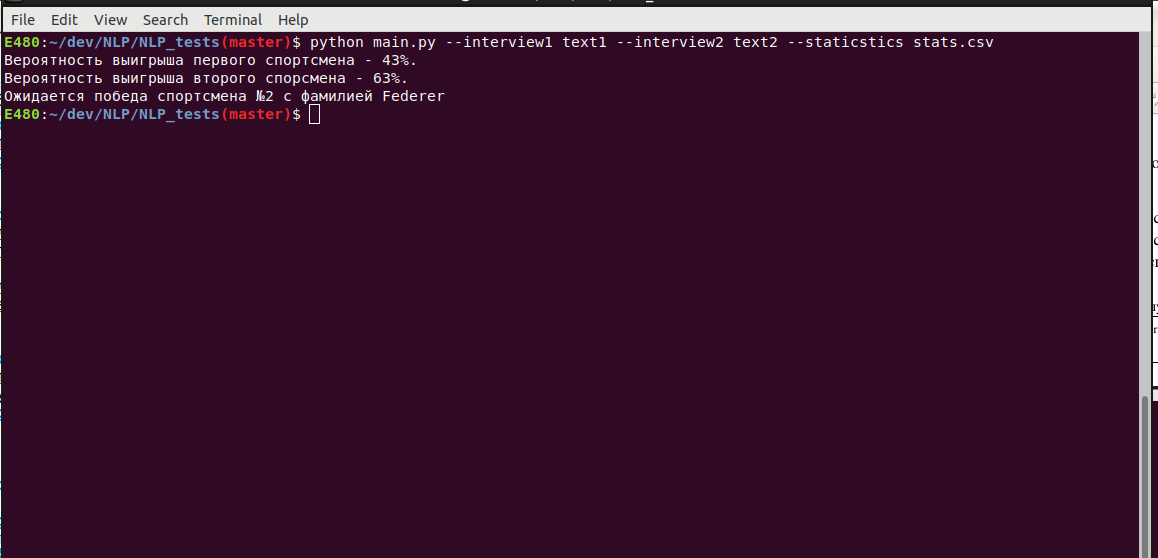
\includegraphics[scale=0.5]{master_img/sample_program.png}
	\caption{Пример работы программы}
	\label{fig10}
\end{figure}